Let us now use mathematical notation and some key equations to present what are perhaps the three most popular elementary machine learning and deep learning models. Note that as is common in mathematical texts, formulas and equations are numbered as (1), (2), etc. and are referenced as such. Models I and II are shallow neural networks and are considered as basic machine learning (and statistical) models. Model~III generalizes these models to a deep neural network and is the archetypal deep learning model.

One of our purposes in this presentation is that the reader explore the notation via several key equations. On a first reading of this section, the reader should not let the notation intimidate them, as it is expected that much of the notation of the equations may be new or forgotten territory. In places where the reader requires more clarity, it is recommended that the reader treat it as motivation for the sections below, where mathematical background is provided, and the equations from this section are further explained. \\

\noindent
{\bf Model I}: {\bf The sigmoid model also known as the logistic model}. Using equations this model, can be described as,
%
\begin{equation}
\label{eq:first-shallow-view}
\hat{y}=\sigma_{\text{Sig}}\big(\overbrace{b_0+w^\top  x}^{z}\big),
% \hat{y}=\underbrace{\sigma_{\text{Sig}}\left(\overbrace{b+w^\top  x}^{z}\right)}_{a},
\qquad
\text{with}
\qquad
\sigma_{\text{Sig}}(z) = \frac{1}{1+e^{-z}}.
\end{equation}
%
Here the input to the model is a list of $p$ numbers, represented all together as $x$, which we can also call a vector, and denote as $x\in {\mathbb R}^p$. The parameters of the model are the number (scalar) $b_0$ which is called the {\em bias}, also known as the intercept, and the vector $w\in {\mathbb R}^p$, which is called the vector of {\em weights}. The operation $b_0 + w^\top x$ means adding the scalar $b_0$ to the inner product operation, $w^\top x$, which also computes to a scalar. We use the overbrace to denote the outcome of this operation as $z$ $=b_0+w^\top x$. Note that this addition of a bias to an inner product is sometimes called an {\em affine transformation}, and can also be written as,
%
\begin{equation}
\label{eq:smallz-only-log-mult}
z = b_0 + \underbrace{\sum_{i=1}^p w_i x_i}_{w^\top x}.
\end{equation}

\begin{figure}[h]
\begin{center}
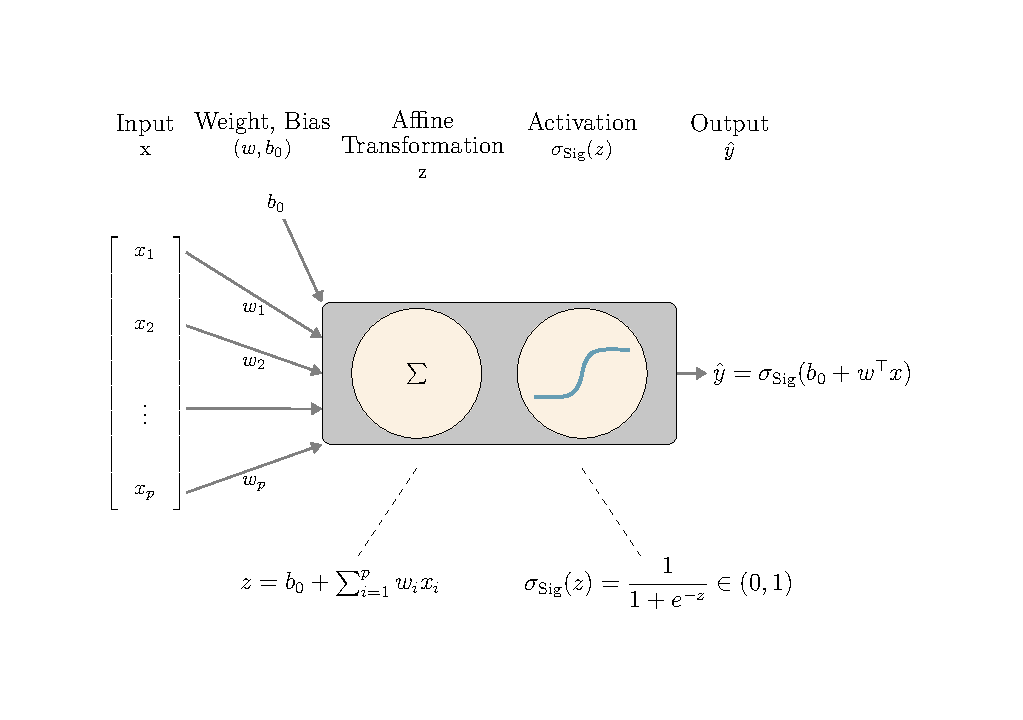
\includegraphics[scale=0.8, trim=0 50 0 50, clip]{../supporting_files/figures/logistic_architecture_chapter_book.pdf}
\end{center}
\caption{The sigmoid model represented with neural network terminology as a shallow neural network. Observe that the artificial neuron is composed of an affine transformation using $z = b_0 + w^\top x$ followed by a non-linear activation transformation 
$\sigma_{\text{Sig}}(z)$.} %The gray box represents an artificial neuron composed of an affine transformation to create $z$ and an activation $\sigma_{\text{Sig}}$.}
\label{fig:niceneuron}
\end{figure}

If the model would have not had $\sigma_{\text{Sig}}(~)$, then it would be a {\em linear model}, which we do not cover here. But with it, the $\sigma_{\text{Sig}}(~)$ means a sigmoid function, which takes any scalar input $z$ and produces a probability output $\hat{y}=\sigma_{\text{Sig}}(z)$. The reader can experiment to compute $1/(1+e^{-z})$ with a calculator or spreadsheet for several values of $z$, to see that it always yields numbers that are between $0$ and $1$, and for example with $z=0$ we have $\sigma_{\text{Sig}}(0) = 1/2$. In a deep learning framework, the function, $\sigma_{\text{Sig}}(~)$, is a type of {\em activation function} and the form of \eqref{eq:first-shallow-view} represents an \textit{artificial neuron} which we also present in Figure~\ref{fig:niceneuron}. 


The sigmoid model can be viewed as the simplest non-linear neural network model. %Outside of the context of deep learning, sigmoid model is known as logistic regression and it is also a very popular statistical model \sbmc{[logistic model is a statistical model. This sentence seems to imply differently. How about "
Outside of the context of deep learning, the sigmoid model is very popular in statistics, and known as {\em logistic regression}. This model is suitable for binary classification tasks where \texttt{positive} samples are encoded via $y=1$ and \texttt{negative} samples are encoded via $y=0$.  The output of the model $\hat{y}$ is a number in the continuous range $[0,1]$ indicating the probability that the features vector $x$, matches a \texttt{positive} label. Hence, the higher the value of $\hat{y}$, the more likely it is that the label associated with $x$ is $y=1$. A classifier can be constructed via a \textit{decision rule} based on a threshold $\tau$, with the predicted output being,
%
\begin{equation} %QQQQ - argue/discuss the order
\label{eq:y-hat-tau}
\widehat{\cal Y} = 
\begin{cases}
0~ (\texttt{negative}), & \text{if} \quad  \hat{y} \le \tau \\
1~ (\texttt{positive}), & \text{if} \quad   \hat{y} > \tau.
\end{cases}
\end{equation}
In many cases one selects the threshold at $\tau = 0.5$. \\

\noindent
{\bf Model II}: {\bf The softmax model also known as the multinomial regression model.} Using equations, this model can be described as,

%
\begin{equation}
\label{eq:softeq}
\hat{y}=S_{\text{Softmax}} \big(\overbrace{b+W  x}^{\quad \,\,\, \, \,\, z\, \in \, {\mathbb R}^K}\big),
% \hat{y}=\underbrace{S_{\text{softmax}} \big(\overbrace{b+W  x}^{z\in {\mathbb R}^K}\big)}_{a\in {\mathbb R}^K},
% \end{equation}
%
\qquad
\text{with}
\qquad
%
% \begin{equation}
% \label{eq:softmax-in-mult}
S_{\textrm{Softmax}}(z) = \frac{1}{\sum_{i=1}^{K} e^{z_i}} 
\begin{bmatrix}
e^{z_1} \\
\vdots\\
e^{z_{K}}\\
\end{bmatrix}.
\end{equation}
%
Here like the sigmoid model, the input, denoted $x$, is a vector of dimension $p$, and as before we can denote this as  $x\in {\mathbb R}^p$. However the output, $\hat{y}$ is no longer a single probability, as in Model~I, but is rather a vector of probabilities of length $K$, where the individual probabilities sum up to $1$. The parameters of the model are also different. The parameter $b$ plays the role of $b_0$ from Model~I and is no longer a scalar, but is rather a vector of dimension $K$, and we denote this as $b\in {\mathbb R}^K$. It is called the {\em bias vector}. As for the weights, unlike Model~I where the weights were in a vector, here we have a matrix of weights, or {\em weight matrix}, $W$, of dimensions $K$ and $p$, where $K$ is the number of matrix rows, and $p$ is the number matrix columns. This can be denoted as $W\in {\mathbb R}^{K\times p}$.

Like Model~I in \eqref{eq:first-shallow-view}, here, the operation of the model in \eqref{eq:softeq} denotes an intermediate variable $z$. The difference is that $z$ is a vector of dimension $K$, denoted $z \in {\mathbb R}^K$. Here to construct $z$ we add the vector $b$ to the vector produced by the matrix-vector multiplication $W x$. 
%, a weight matrix of numbers are the parameters of the model. The input $x\in {\mathbb R}^p$ is also a vector, and $b + Wx$ means the matrix-vector multiplication ($Wx$), followed by the vector-vector addition (adding $b$). 
This means that for $i=1,\dots,K$, each scalar, $z_i$ in the vector $z\in {\mathbb R}^K$ is computed as,
%
\begin{equation}
\label{eq:small-zk-log-mult}
z_i = b_i + \sum_{j=1}^p w_{i,j} \, x_j,
\end{equation}
%
where $b_i$ is the $i$-th scalar in the vector $b$ and $w_{i,j}$ is the scalar in the matrix $W$ at row $i$ and column $j$.

Like Model~I, that applies the (non-linear) function $\sigma_{\text{Sig}}(~)$ on the scalar $z$, here with Model~II we apply the function $S_{\textrm{softmax}}(~)$ on the vector $z$. This function is called the {\em softmax} and it converts a vector of dimension $K$ to a different vector of the same dimension $K$, where all elements of the output vector are probabilities, and they sum up to $1$.

\begin{figure}[h]
\begin{center}
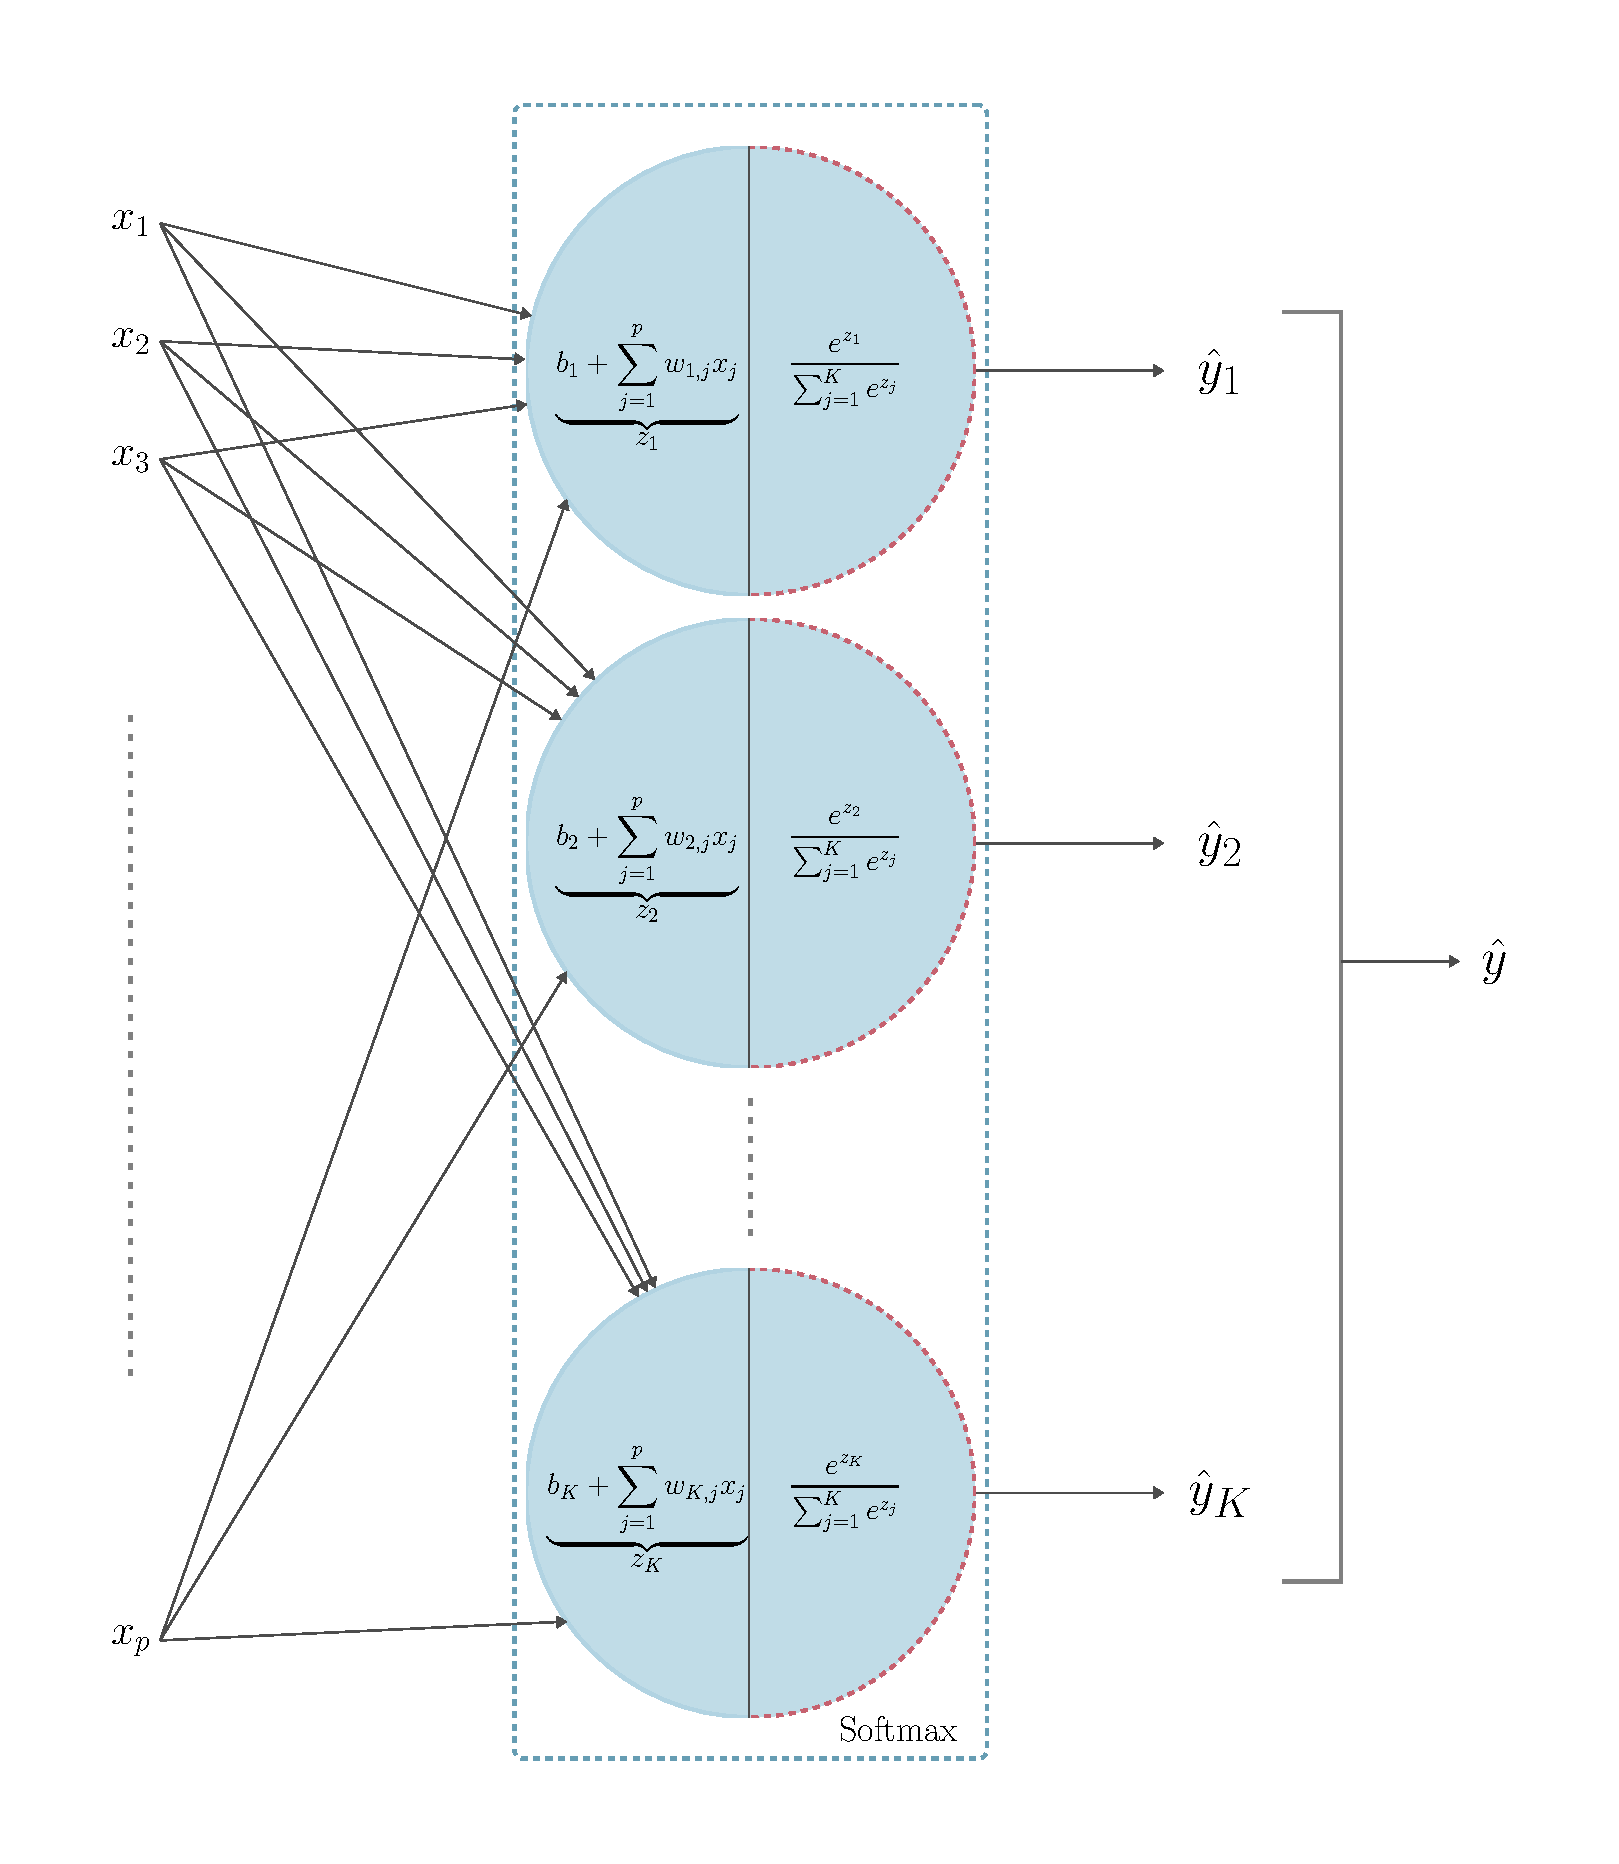
\includegraphics[scale=0.48,trim=50 50 50 50, clip]{../supporting_files/figures/figure_softmax.pdf}%softmax_layer.pdf}
\end{center}
\caption{The softmax model as a shallow neural network model with output $\hat{y}$ which is composed of elements $\hat{y}_1, \ldots, \hat{y}_K$,  representing a probability vector. }
\label{fig:shalsoft}
\end{figure}

The form of \eqref{eq:softeq} positions the softmax model as a shallow neural network similarly to the way that the sigmoid model is a shallow neural network. The difference is that the softmax model has vector outputs while the sigmoid model has a scalar output. Figure~\ref{fig:shalsoft} illustrates the softmax model as a neural network. Here each circle can again be viewed as an ``artificial neuron'' however note that the softmax function %\sbmc{[note that the phrase 'activation' is used first time here for this model.]} 
affects all neurons together via the normalization in the denominator of the softmax function $S_{\textrm{softmax}}(~)$. Hence the activation value of each neuron is not independent of the activation values of the other neurons.

The softmax model, also known as the multinomial regression model, is the most popular model for multi-class classification, where the goal is to provide a prediction $\widehat{\cal Y}$ for the label in $\{1,\ldots,K\}$ associated with the input feature vector $x$.  The softmax model produces an output vector, $\hat{y}$, which is a probability vector, and can be used to create a classifier by choosing the class that has the highest probability. Namely,
%
\begin{equation}
\label{eq:argmax-mp}
\widehat{\cal Y}=\underset{k \in\{1, \ldots, K\}}{\operatorname{argmax}} ~\hat{y}_k,
\end{equation}
%
and this means to choose the index $k$ from the set $\{1,\ldots,K\}$, where the entry (probability) $\hat{y}_k$ is highest. 
This approach is called a \textit{maximum a posteriori probability} (MAP) decision rule since it simply chooses $\widehat{\cal Y}$ as the class that is most probable. It is the most common decision rule when using deep learning models for classification. \\

\noindent
{\bf Model III}: {\bf General fully connected neural networks also known as feedforward networks.} Using equations, this model can be described as,
%
\begin{equation}
\label{eq:generalRecursiveModel}
\hat{y}=f^{[L]}(f^{[L-1]}(f^{[L-2]}(\ldots (f^{[1]}(x))\ldots))),
% f_{\mathbf{\theta}}(x)=f_{\mathbb{\theta}^{[L]}}^{[L]}(f_{\mathbb{\theta}^{[L-1]}}^{[L-1]}(\ldots (f_{\mathbb{\theta}^{[1]}}^{[1]}(x))\ldots)),
\end{equation}
%
where each individual function $f^{[\ell]}(~)$ operating on some input $u$, can be  described as,
%
\begin{equation}
\label{eq:dense-layer}
f^{[\ell]}(u) =
S^{[\ell]}(b^{[\ell]} + W^{[\ell]} u),
\qquad
\text{for}
\qquad
\ell = 1,\ldots,L.
\end{equation}
%
Here in \eqref{eq:generalRecursiveModel} we see composition of functions, where first the function $f^{[1]}(~)$ is applied to the input $x$, and then the function $f^{[2]}(~)$ is applied on the output of $f^{[1]}(x)$, and then $f^{[3]}(~)$ is applied on the output of $f^{[2]}(f^{[1]}(x))$, and so fourth until the last function $f^{[L]}(~)$ is applied on what was computed prior. Each such function application is the operation of a {\em layer} in a deep neural network. 

Different types of neural networks have different types of layers, and in the simplest case of feedforward fully connected neural networks, \eqref{eq:dense-layer} describes the operation of layer~$\ell$. Observe that \eqref{eq:dense-layer} is somewhat similar to the left side of \eqref{eq:softeq}. In the case of \eqref{eq:dense-layer}, we have that $S^{[\ell]}(~)$ is some vector activation function, while in the case of \eqref{eq:softeq} there is only a single layer (and hence $\ell$ is absent) and the activation function is the softmax function.  

\begin{figure}[h!] 
\begin{center}
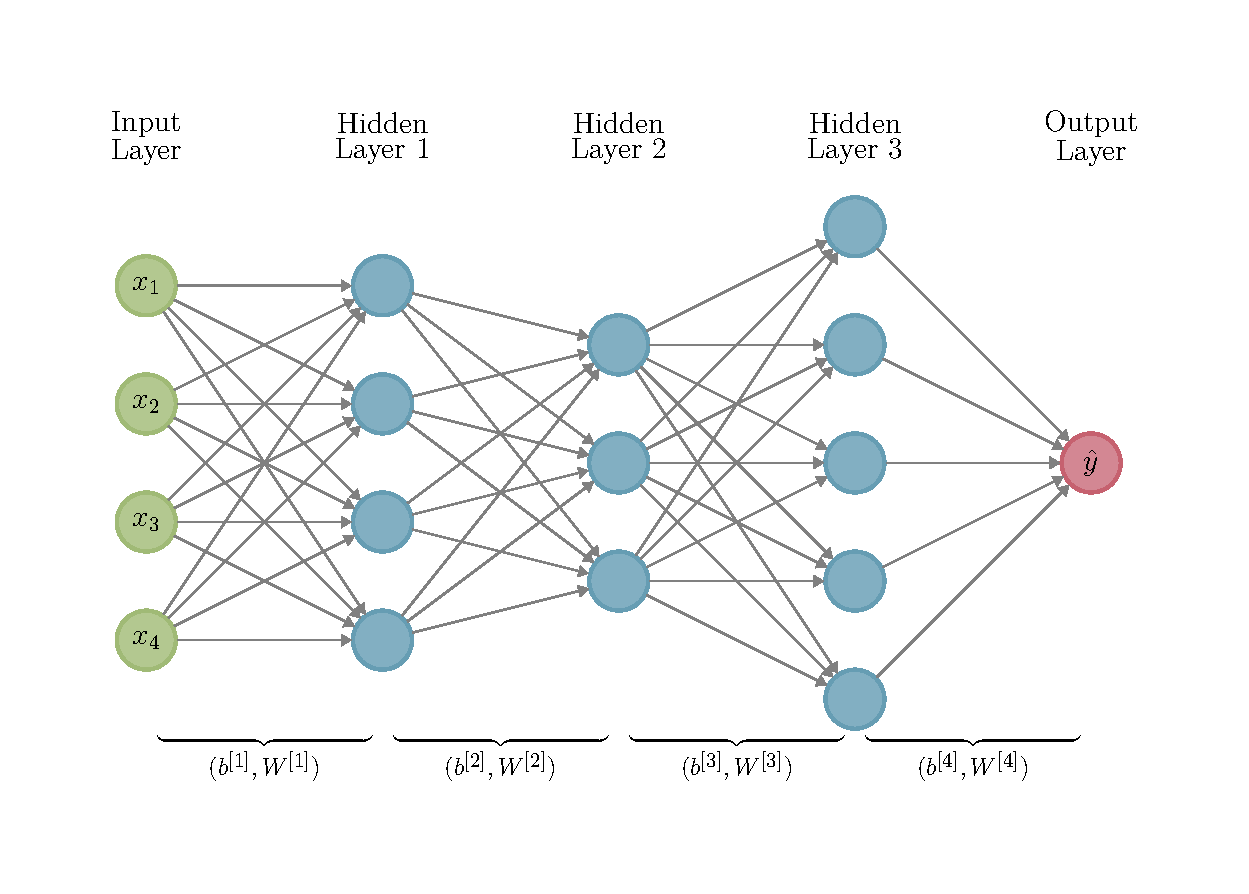
\includegraphics[scale=0.7,trim=0 40 0 50, clip]{../supporting_files/figures/deep_neural_network1.pdf}
 \caption{A fully connected feedforward deep neural network with multiple hidden layers. The input to the network is the vector $x = (x_1, x_2, x_3, x_4)$ and in this case the output is the scalar~$\hat{y}$. For this particular example the dimensions of $W^{[1]}$ are $4\times 4$, $W^{[2]}$ is $3 \times 4$, $W^{[3]}$ is $5 \times 3$, and $W^{[4]}$ is $1 \times 5$. The bias vectors are of dimension $4$ for $b^{[1]}$, $3$ for $b^{[2]}$, $5$ for $b^{[3]}$, and $1$ (a scalar) for $b^{[4]}$.
 }
    \label{FFNN}
\end{center}
\end{figure}

The parameters of each layer $\ell$ are also similar to Model~II (which only has a single layer). Here with Model~III, each layer has a {\em bias vector} $b^{[\ell]}$ and a {\em weight matrix} $W^{[\ell]}$. The dimensions of these vectors and matrices are specific to the architecture of the network, and we fill in these details in Section~\ref{sec:putting-bits-together}. At this point, let us appreciate that Model~III is more complex. For one thing, it has the rich set of parameters $(b^{[1]}, W^{[1]}), \ldots, (b^{[L]}, W^{[L]})$ which can easily involve hundreds of thousands, millions, or billions of individual scalar parameters.  With so many parameters organized in layers, it is generally much more expressive and can capture complex relationships in data. Figure~\ref{FFNN} presents a schematic of such a deep neural network.
